%\begin{CJK*}{GBK}{song}
%\begin{CJK*}{GBK}{kai}
%beamer下不能用\songyi、\zihao等命令!
%\graphicspath{Figures/}

%\renewcommand{\figurename}{\tiny\CJKfamily{hei} 图.}
\renewcommand{\figurename}{\tiny{\bf Fig}.}
%\renewcommand{\tablename}{\tiny\CJKfamily{hei} 表.}
\renewcommand{\tablename}{\tiny{\bf Tab}.}
%\renewcommand{\tablename}{\tiny\CJKfamily{hei} 表.}
%\renewcommand{\thesubfigure}{\roman{subfigure}}  %\makeatletter 子图标记罗马字母
\renewcommand{\thesubfigure}{\tiny(\alph{subfigure})}  %\makeatletter 子图标记英文字母
%\renewcommand{\thesubfigure}{}  \makeatletter %子图无标记

%%%%%%%%%%%%%%%%%%%%%%%%%%%%%%% Latex 的 tikz 绘图 %%%%%%%%%%%%%%%%%%%%%%%%%%%%%%%%%%%%%%%%%%%
%\begin{tikzpicture}
%    % 引入图片
%    \node[anchor=south west,inner sep=0] (image) at (0,0) {\includegraphics[width=0.9\textwidth]{Mycena_interrupta.jpg}};
%
%    \begin{scope}[x={(image.south east)},y={(image.north west)}]
%        % 建立相对坐标系
%        \draw[help lines,xstep=.1,ystep=.1] (0,0) grid (1,1);
%        \foreach \x in {0,1,...,9} { \node [anchor=north] at (\x/10,0) {0.\x}; }
%        \foreach \y in {0,1,...,9} { \node [anchor=east] at (0,\y/10) {0.\y}; }
%        % 作图命令
%        \draw[red, ultra thick, rounded corners] (0.62,0.65) rectangle (0.78,0.75);
%    \end{scope}
%\end{tikzpicture}
%指定位置插入图片
%\begin{tikzpicture}[remember picture,overlay]
%    \node<1->[xshift=-3cm,yshift=-1cm] at (current page.center) {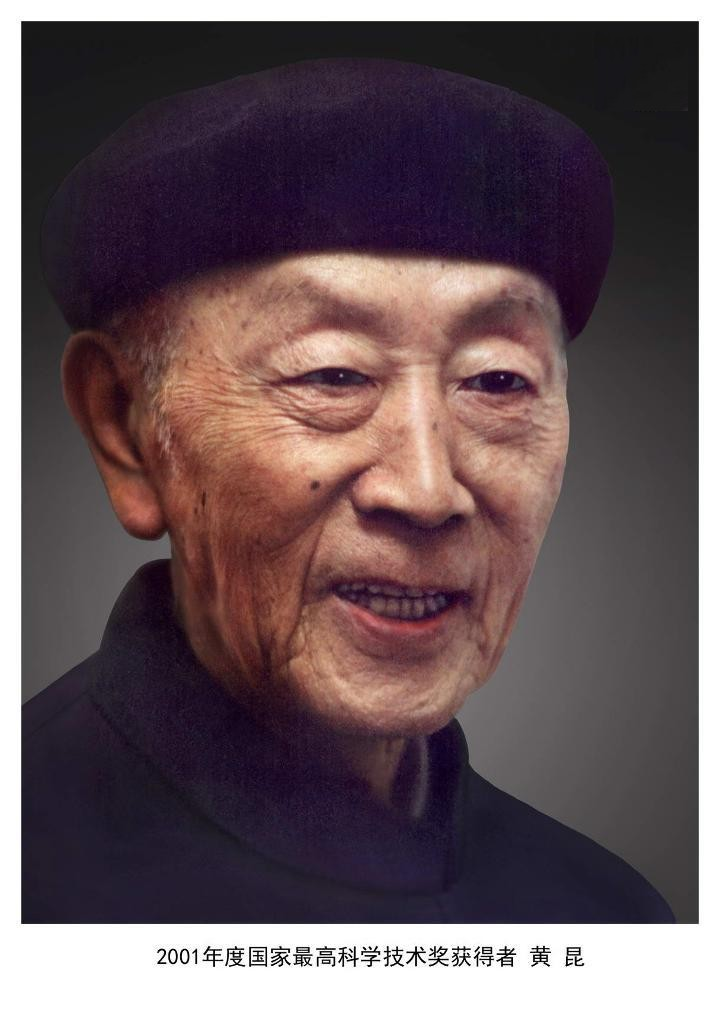
\includegraphics[height=3cm]{Figures/Huang.jpg}};
%    \node<2->[xshift=0cm,yshift=0cm] at (current page.east) {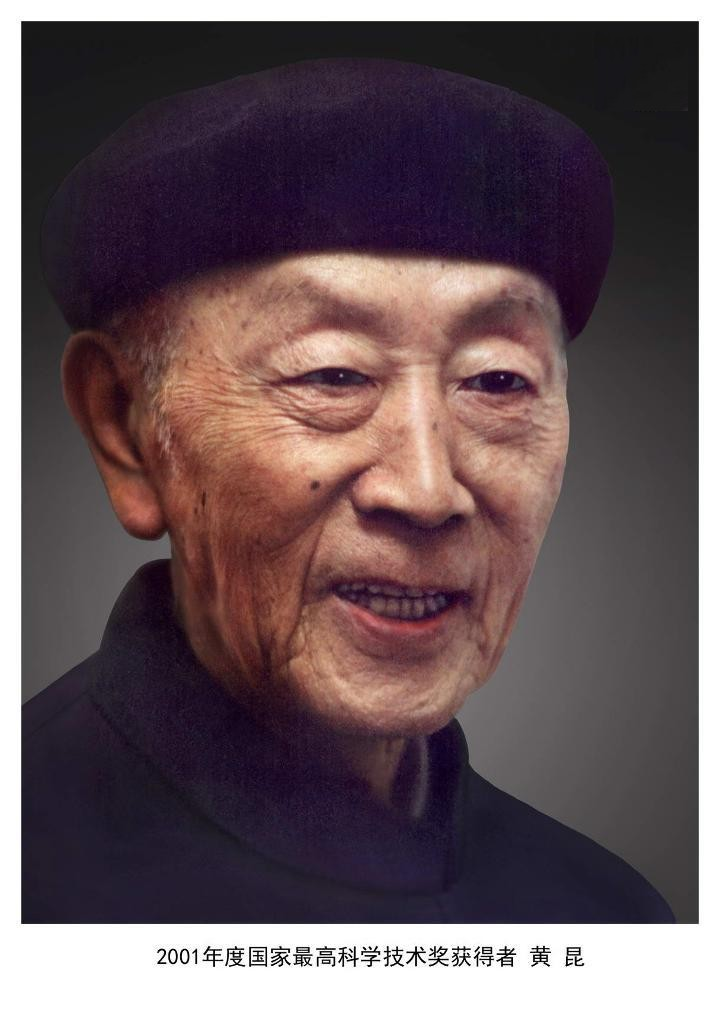
\includegraphics[height=3cm]{Figures/Huang.jpg}};
%    \node<3->[xshift=3cm,yshift=1cm] at (current page.north) {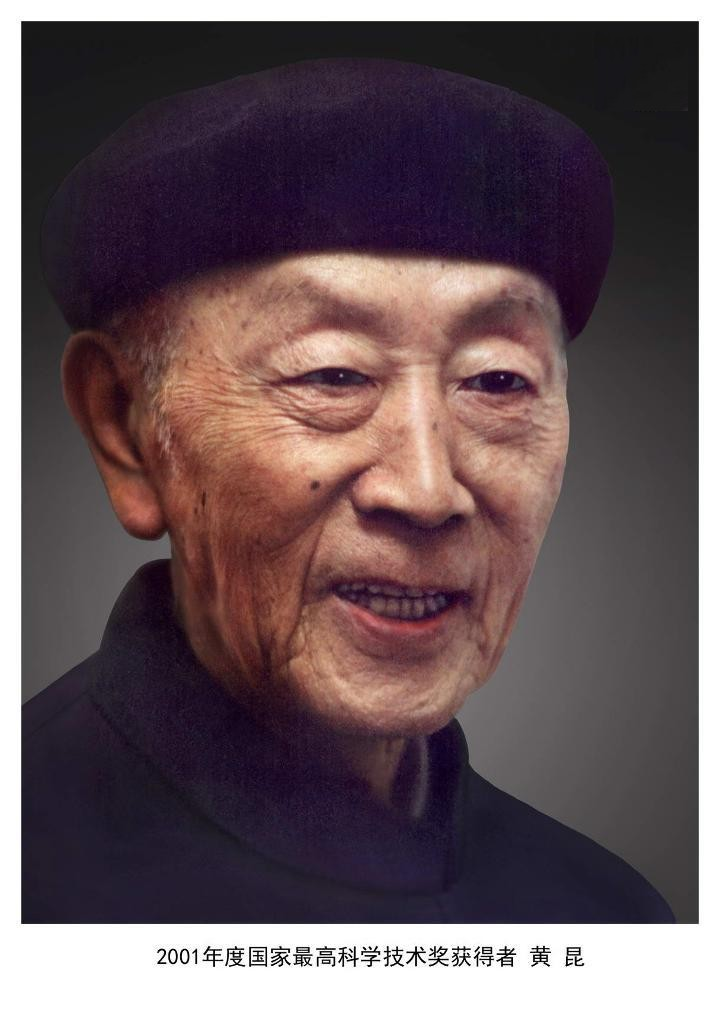
\includegraphics[height=3cm]{Figures/Huang.jpg}};
%\end{tikzpicture}
%\begin{tikzpicture}[remember picture,overlay]
%	\node[xshift=-1.8cm,yshift=1.43cm] at (current page.east) {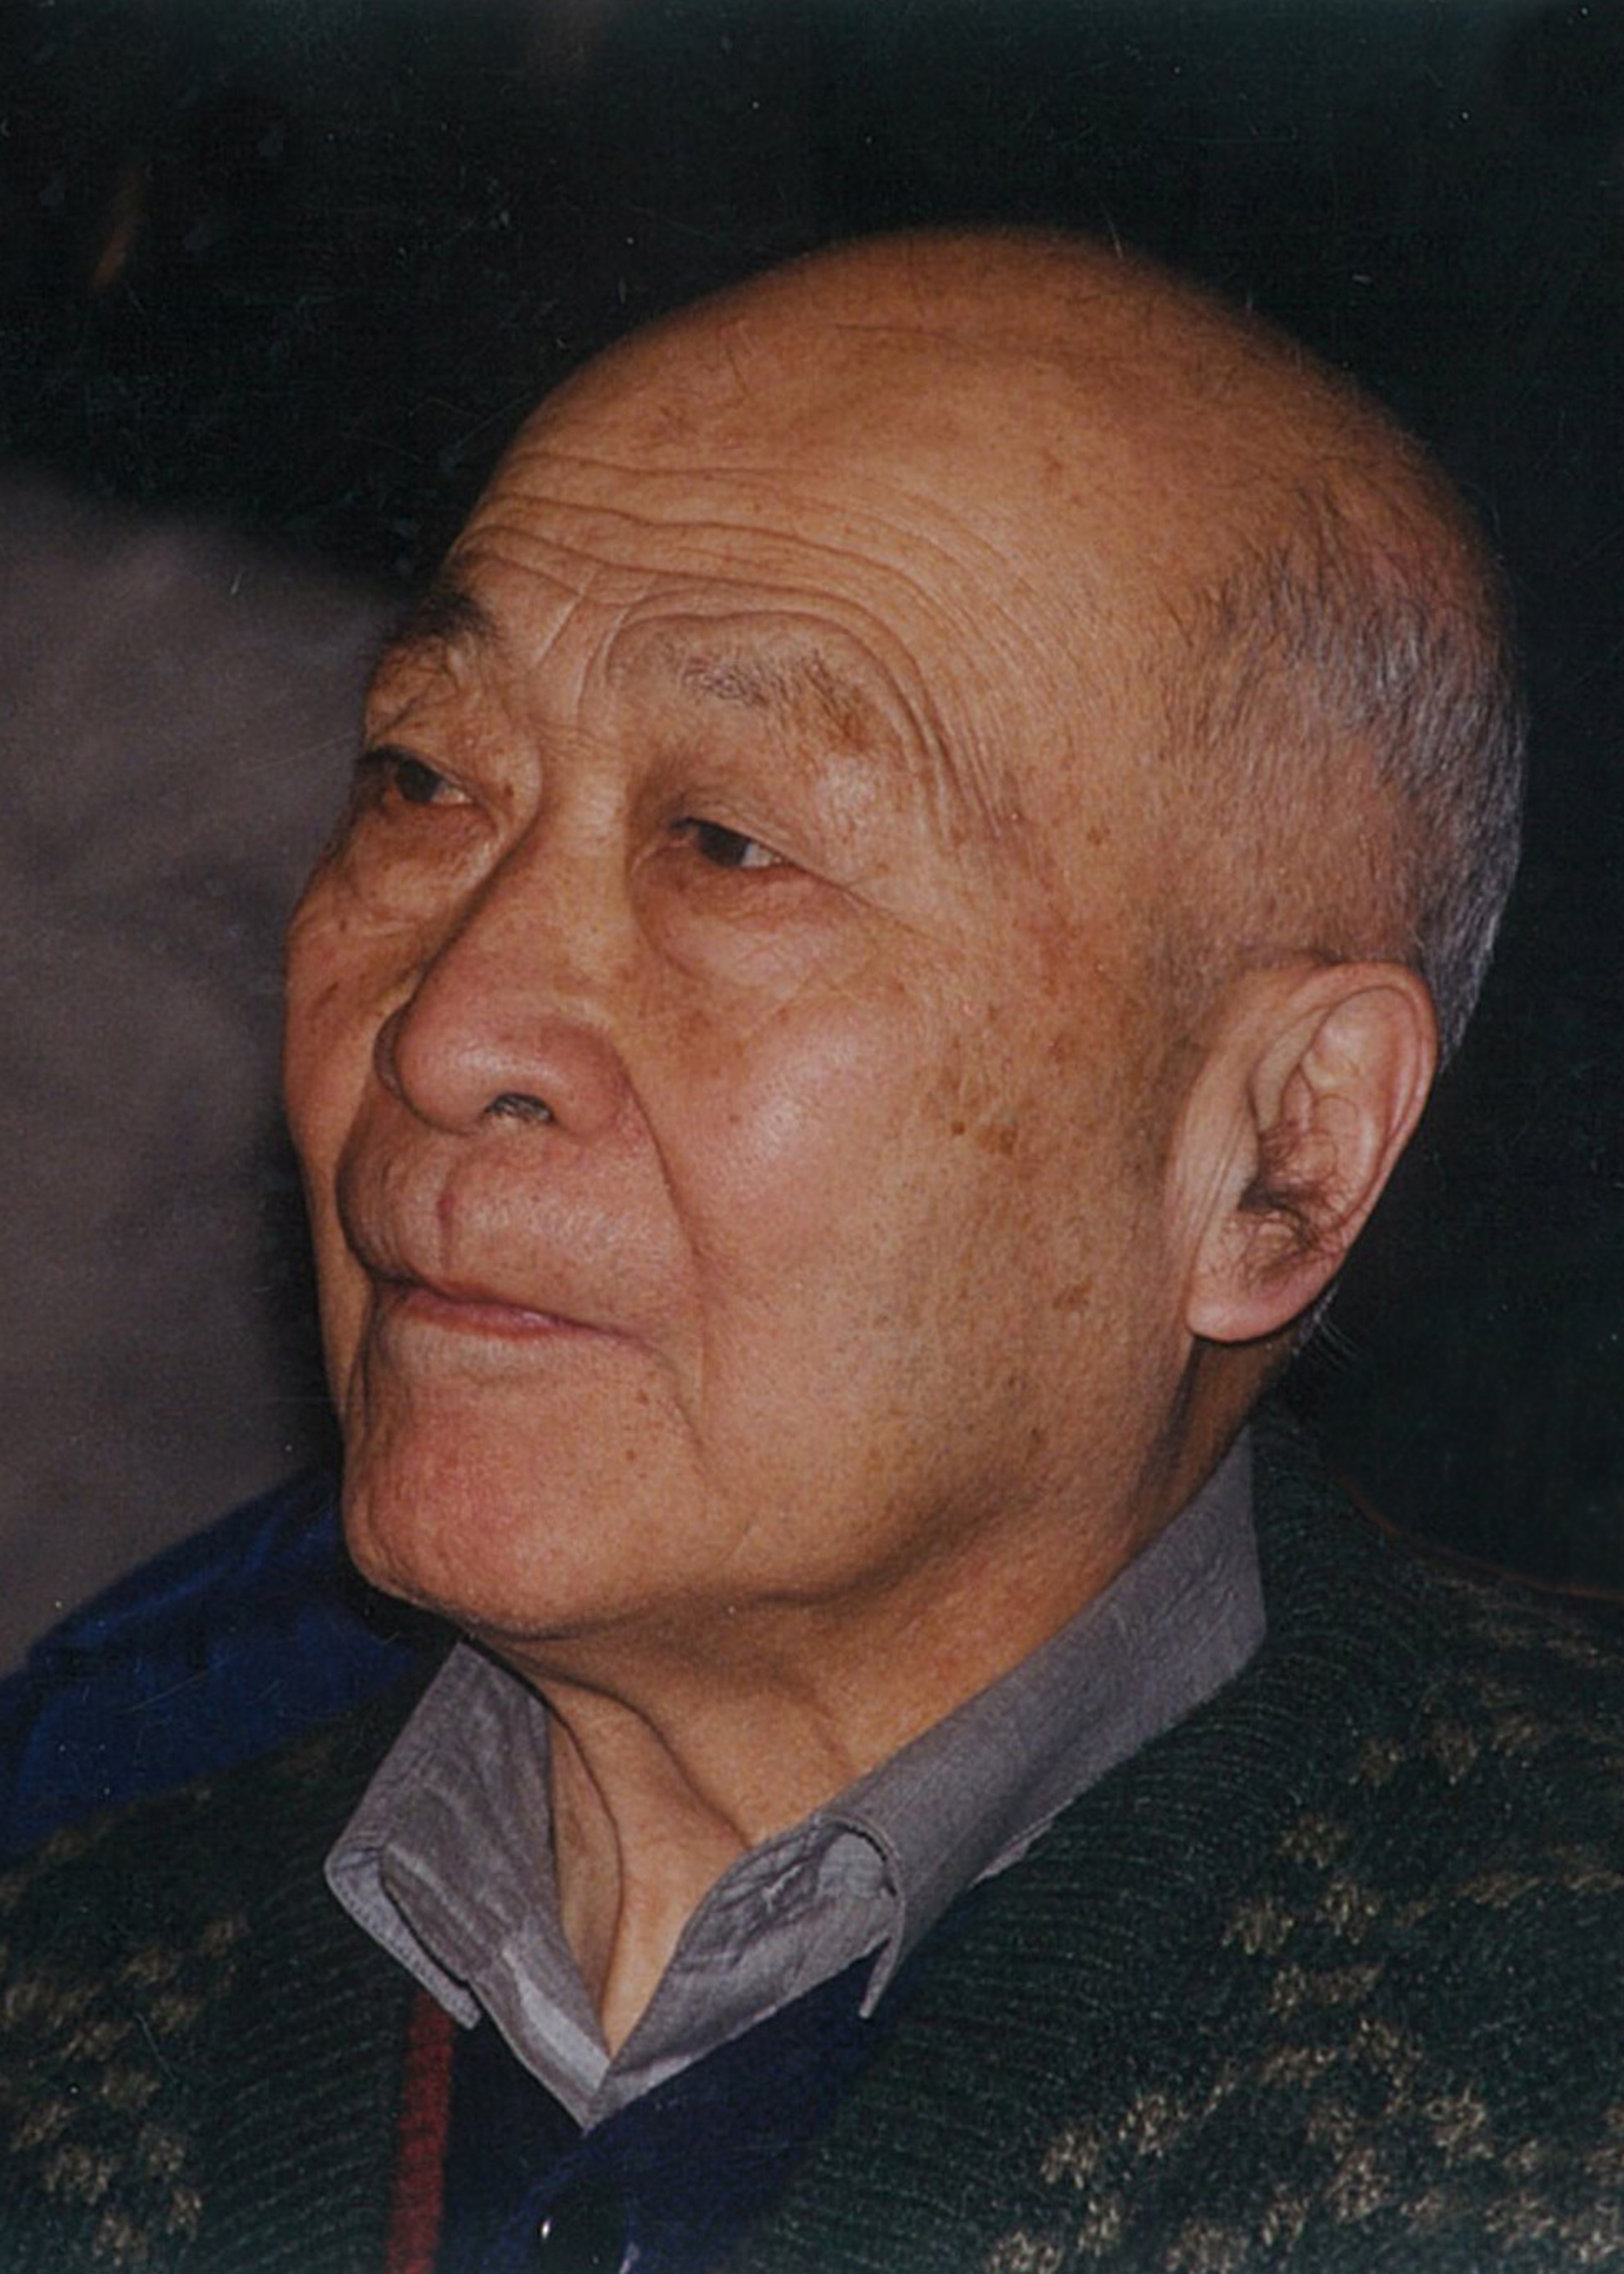
\includegraphics[height=2.5cm, width=2.22cm, viewport=360 0 1350 1100,clip]{Figures/Liu_Zengfu.jpg}};
%\end{tikzpicture}
%常用的位置有 center, north west, west, north, base, north east, east
%%%%%%%%%%%%%%%%%%%%%%%%%%%%%%%%%%%%%%%%%%%%%%%%%%%%%%%%%%%%%%%%%%%%%%%%%%%%%%%%%%%%%%%%%%%%%%

